\chapter{The \chips R\&D Project}
\label{chap:chips}

\section{Things to talk about}

- General overview of why a large, cheap detector like CHIPS is needed
PLOT:
- Brief overview of what CHIPS could add to physics, what it can detect etc...
- general non-detailed description of the general principles behind CHIPS

REF: Hyper-k letter of intent~\cite{abe2011}
REF: Dune CDR~\cite{acciarri2016}

- First how beam water Cherenkov detect events
- Describe the Numi beam
- An aside on the off-axis effect
- Describe the Cherenkov effect
- Describe the flux and expected cross-sections / types of event
- Give the expected number of events that CHIPS should see
- An aside on GENIE which we used for event generation
- Describe all the possible interactions that can be observed in CHIPS
- What are the classic difficulties with water Cherenkov detectors
- Brief description of how PMTs detect the cherenkov light
- CHIPS detector simulation
- Example plots of events for different signature types of events...

- The CHIPS-M detector and conclusions

- The CHIPS-10 detector
- General structure, how it all holds together
- How it is deployed/extended
- How it detects the Cherenkov light with PMTs arranged in planes
- How the construction went
- Current status and future plans

- The tau neutrino component is negligible and not predicted by the simulation

\section{Diagrams}

- Overhead shot, with depth contours and detector location in the pit
\begin{figure}
    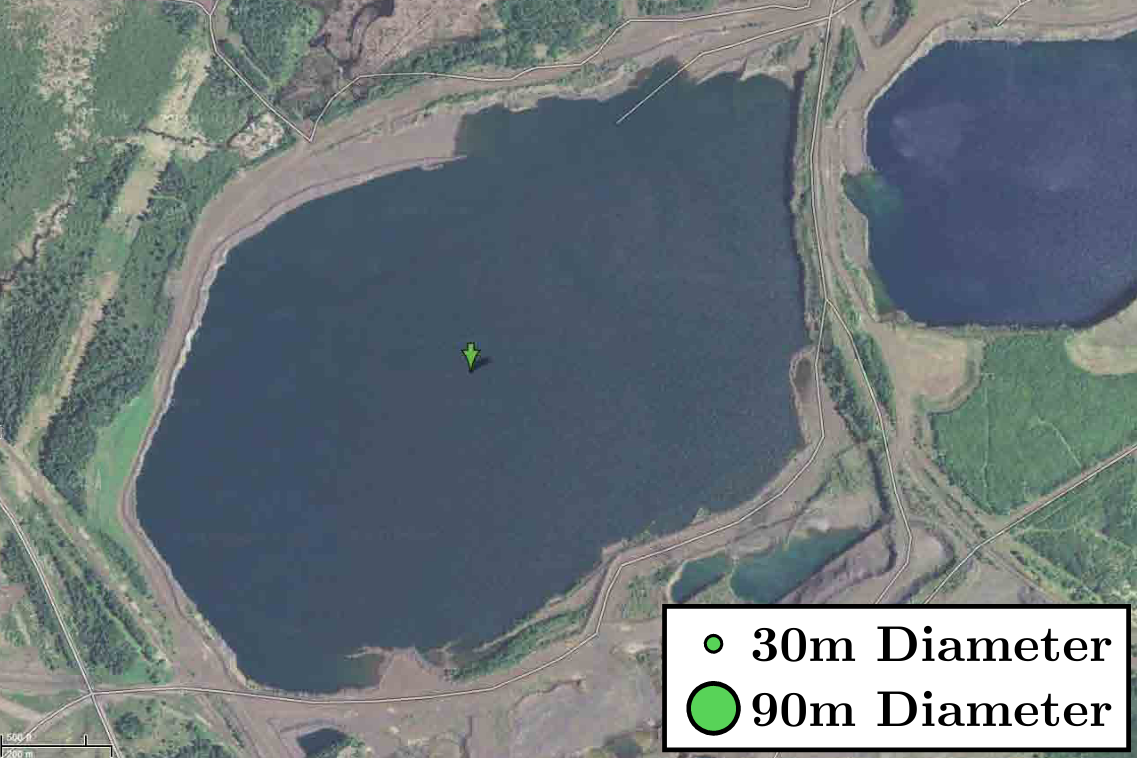
\includegraphics[width=\textwidth]{diagrams/4-chips/location.png}
    \caption[location short]{location long}
    \label{fig:location}
\end{figure}
- Topological plot overhead (contours)
\begin{figure}
    \includegraphics[width=\textwidth]{diagrams/4-chips/contour_map.pdf}
    \caption[contour map short]{contour map long}
    \label{fig:contour_map}
\end{figure}
- CHIPS-M detector picture
\begin{figure}
    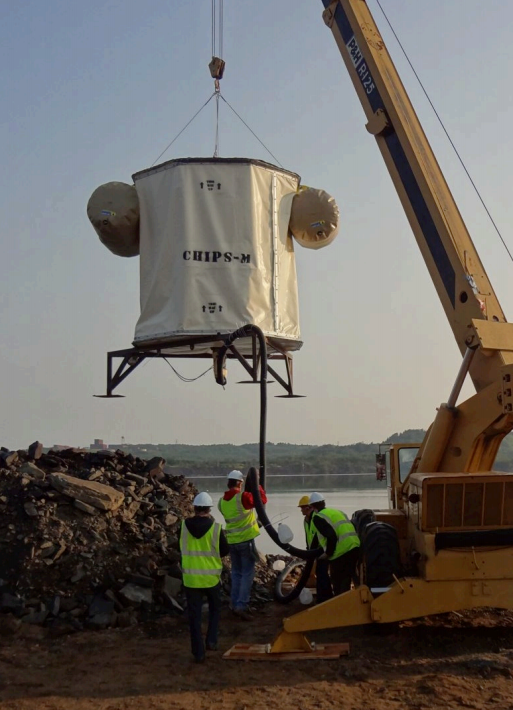
\includegraphics[width=0.8\textwidth]{diagrams/4-chips/chips_m.png}
    \caption[chips m short]{chips m long}
    \label{fig:chips_m}
\end{figure}
- CHIPS Render
\begin{figure}
    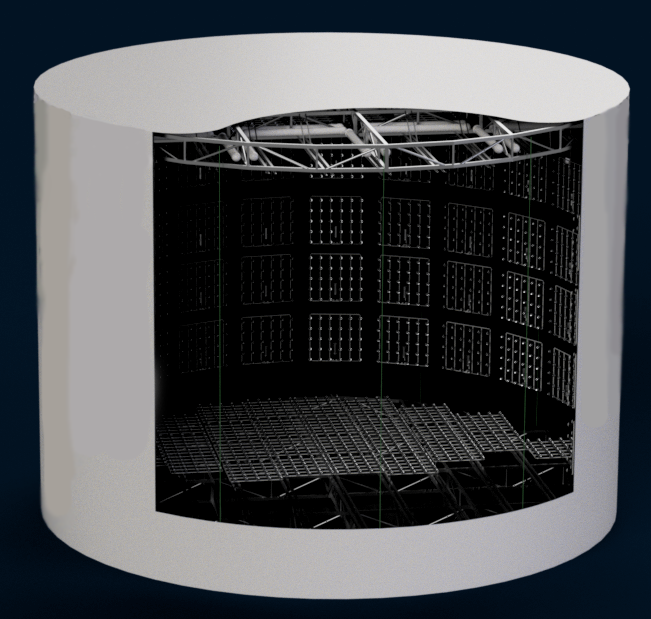
\includegraphics[width=\textwidth]{diagrams/4-chips/chips_render_1.png}
    \caption[chips render 1 short]{chips render 1 long}
    \label{fig:chips_render_1}
\end{figure}
\begin{figure}
    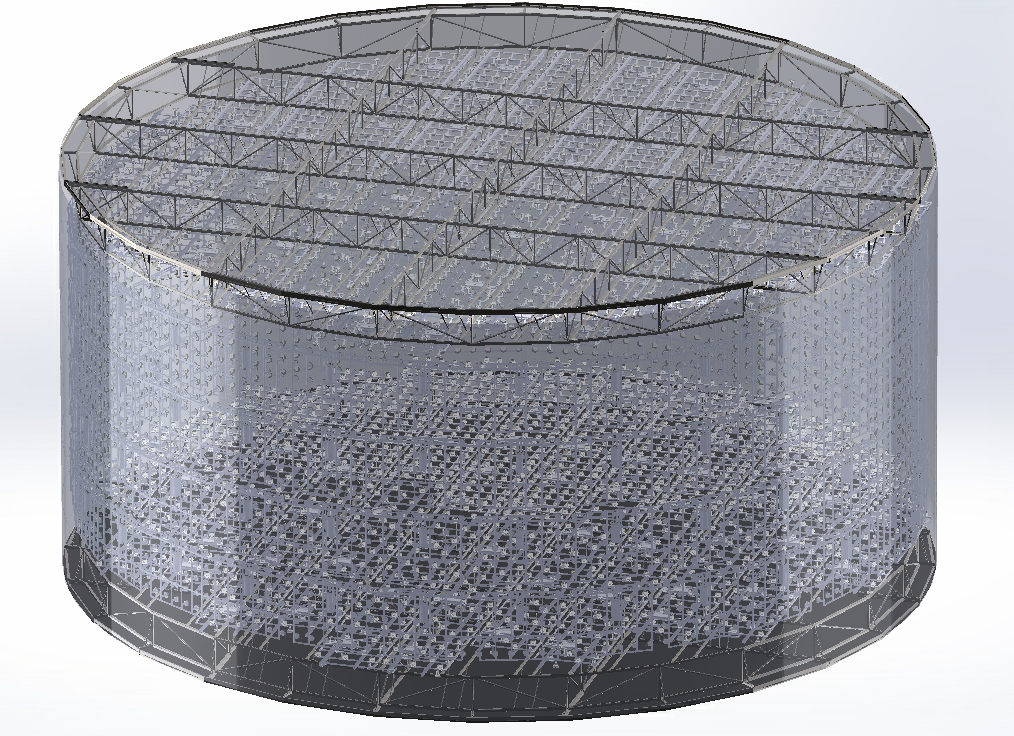
\includegraphics[width=\textwidth]{diagrams/4-chips/chips_render_2.png}
    \caption[chips render 2 short]{chips render 2 long}
    \label{fig:chips_render_2}
\end{figure}
- General metal frame structure diagram
- POM diagram
- Cosmic rate given the water overburden diagram
- Chips fiducial volume diagram with dimensions around the sides
- CHIPS expected event rate plot with and without oscillations
- CHIPS location in numi
\begin{figure}
    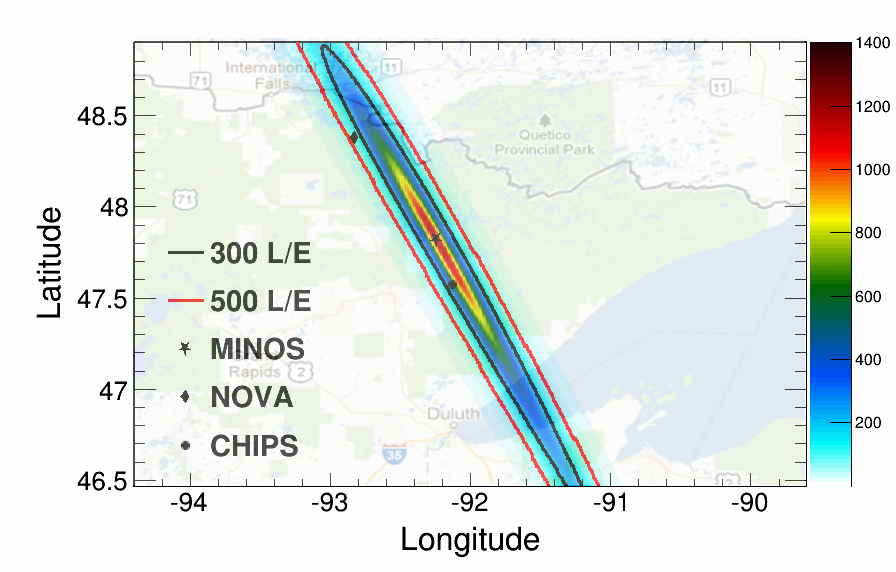
\includegraphics[width=\textwidth]{diagrams/4-chips/numi_map.png}
    \caption[numi map short]{numi map long}
    \label{fig:numi_map}
\end{figure}
- Numi beam pipe diagram
\begin{figure}
    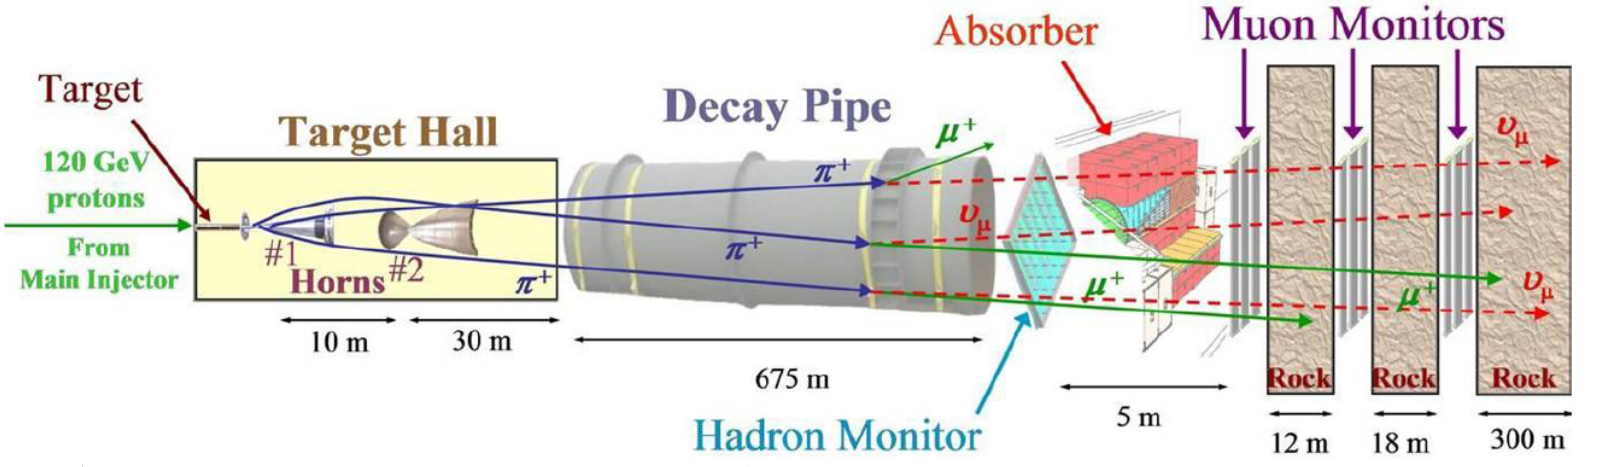
\includegraphics[width=\textwidth]{diagrams/4-chips/numi_beam.png}
    \caption[numi beam short]{numi beam long}
    \label{fig:numi_beam}
\end{figure}
- Off-axis, minos vs chips vs nova plot
\begin{figure}
    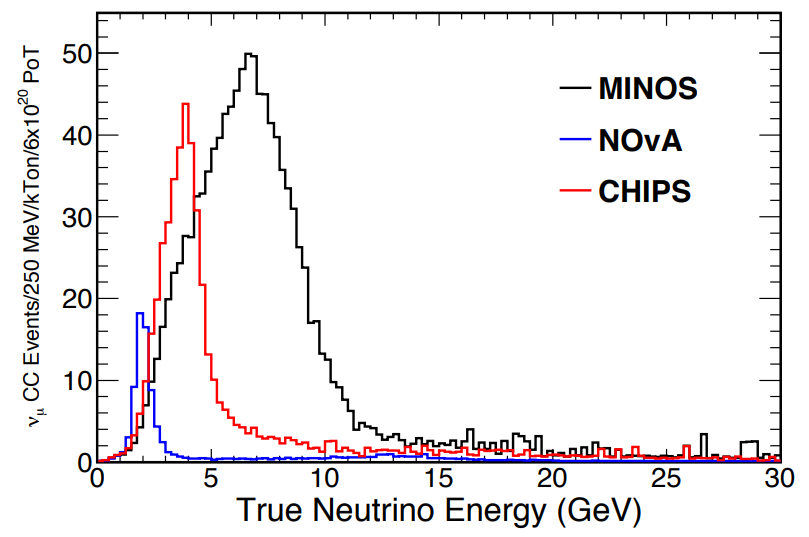
\includegraphics[width=\textwidth]{diagrams/4-chips/numi_axis.png}
    \caption[numi axis short]{numi axis long}
    \label{fig:numi_axis}
\end{figure}
- Numi CHIPS flux
\begin{figure}
    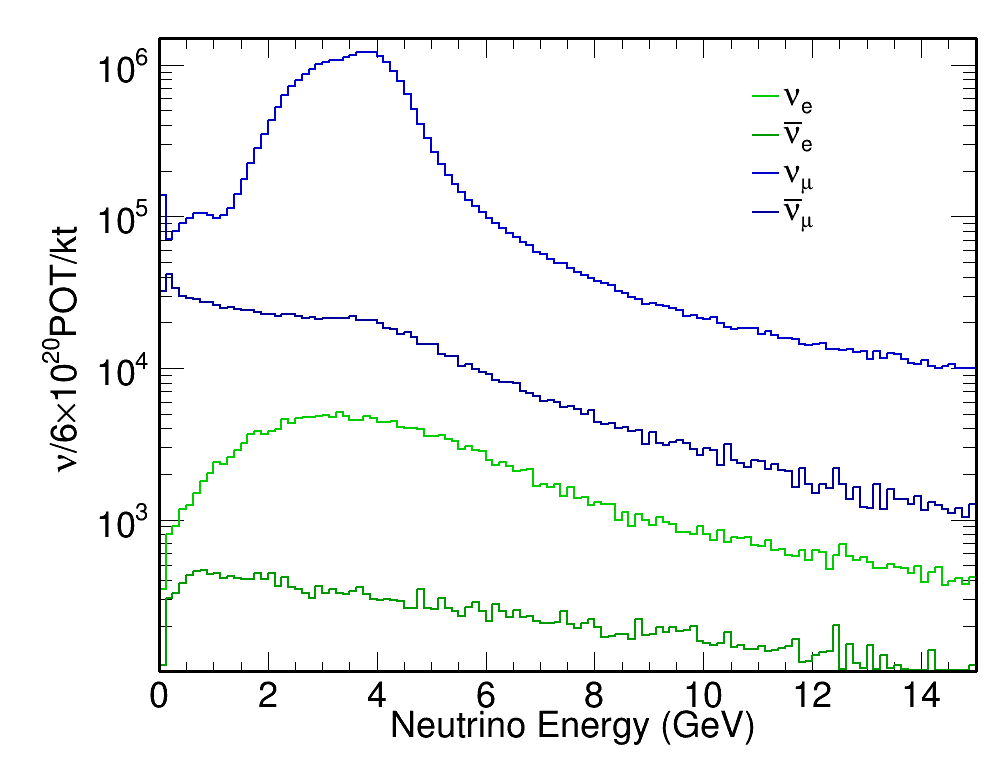
\includegraphics[width=\textwidth]{diagrams/4-chips/flux.png}
    \caption[flux short]{flux long}
    \label{fig:flux}
\end{figure}
- Event in CHIPS simulation
\begin{figure}
    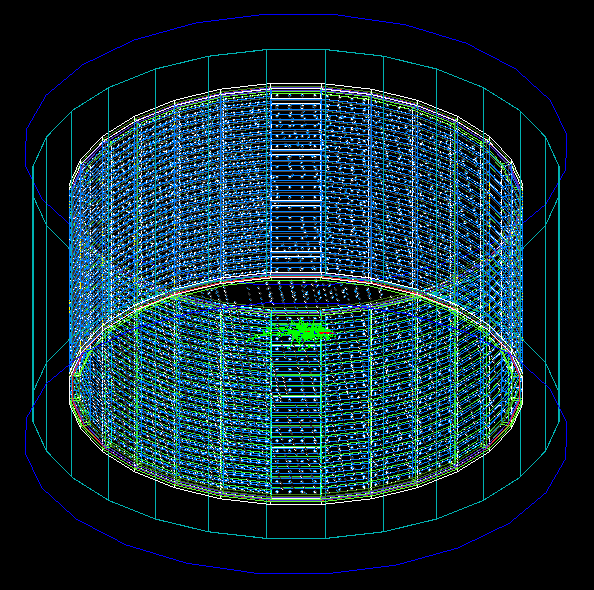
\includegraphics[width=\textwidth]{diagrams/4-chips/chips_event.png}
    \caption[chips event short]{chips event long}
    \label{fig:chips_event}
\end{figure}
- Cherenkov effect diagram
- Floating dock diagram
- deployment diagram
- Simulated events for different types
- Cosmics around chips
\begin{figure}
    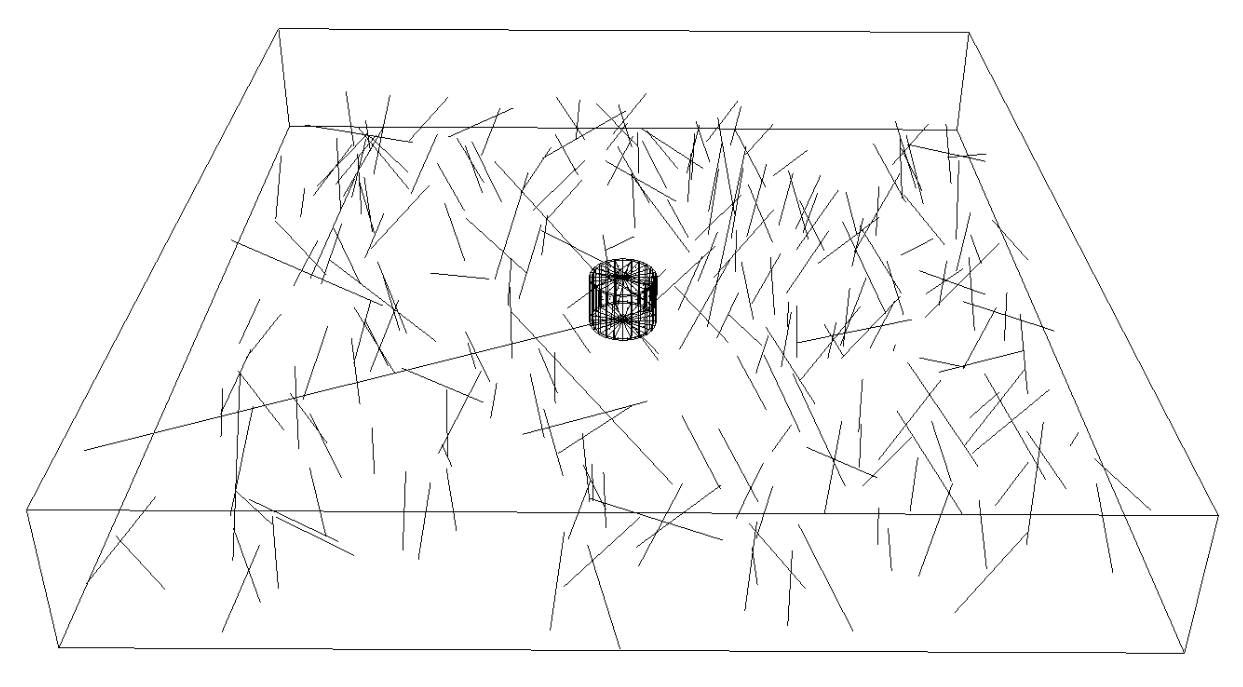
\includegraphics[width=\textwidth]{diagrams/4-chips/cosmics.png}
    \caption[cosmics short]{cosmics long}
    \label{fig:cosmics}
\end{figure}


\section{References}


- CHIPS letter of intent~\cite{adamson2013}
- CHIPS attenuation length paper~\cite{amat2017}
- CHIPS reco paper~\cite{blake2016}
- Karol prospects for CHIPS paper~\cite{lang2015}
- Andy CHIPS-M prototype construction and simulations~\cite{perch2015}
- Maciej prototype detection unit~\cite{pfutznerProto2017}
- Sensitivity Determination in the CHIPS Neutrino Detector~\cite{adde2016}
- The Numi beam big paper~\cite{adamson2016}
- Icecube DOM paper
- km3net General paper
- Km3net optical module paper
- Nemo-3 PMT paper


\section{Reference notes}

